\documentclass[border=1pt]{standalone}
\usepackage{tikz}
\usepackage{luatexja}

\begin{document}
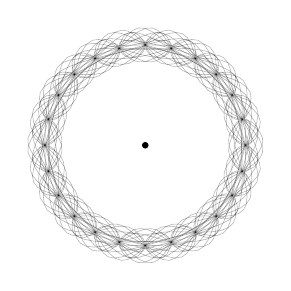
\begin{tikzpicture}[scale=1.5]
    % 補助的な円（波の広がりを感じさせる）
    \draw[black!5, line width=0.1pt] (0,0) circle (0.85);
    
    % 波動の干渉を描写
    \foreach \i in {1,2,...,24}{ % 本数を増やして密度をさらにアップ
        \draw[black, opacity=0.3, line width=0.2pt, rotate=\i*15] 
            plot[domain=0:2*pi, samples=100] ({0.85*cos(\x r)}, {0.15*sin(6*\x r) + 0.85*sin(\x r)});
    }
    
    % 中央にアクセント（粒子の性質を象徴する点）
    \fill[black] (0,0) circle (0.8pt);
        
\end{tikzpicture}
\end{document}
